\documentclass[a4paper]{article}
\usepackage{graphicx}
\usepackage[utf8]{inputenc}

\title{Assignment 00 - BDSA}
\author{Asmus Tørsleff}
\begin{document}

\maketitle

\section{The Algorithm}
In the diagram below the Main and IsLeapYear methods are described as one process. We find out if the number is divisible by anding it with the bit mask 0b11 to check if the last 2 bits are set, if they are not, the number is divisible by 4 in the same way any number in base 10 that does not end with 0 is not divisible by 10. We use the modulo operator for the other two checks. If it the fist condition is true and either of the other two conditions are true we print "Yay!", otherwise we print "Nay!"

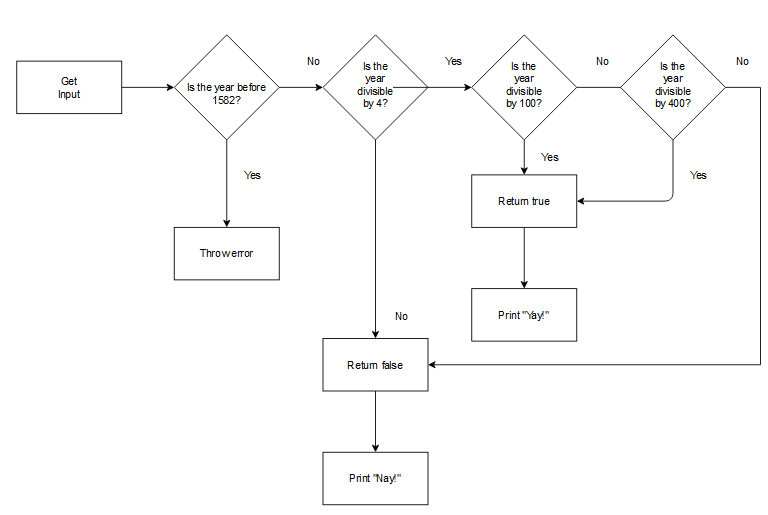
\includegraphics[width = \linewidth]{Documentation/Flowchart.PNG}
\end{document}
\documentclass{article}

